Una de las grandes contribuciones de la ciencia fue el desarrollo de la máquina calculadora. La primera calculadora mecánica de la historia, conocida como Pascalina, fue inventada por el francés \textit{Blaise Pascal}. Fue el joven a la edad de diecinueve años, en 1642, cuando este inventó una máquina que era capaz de realizar sumas, restas hasta incluso multiplicar y dividir mediante restas y sumas sucesivas. Este tuvo una gran repercusión computacional tanto es así que aún sigue teniendo influencia en nuestros días. A continuación se muestra una imagen de dicha calculadora.

\begin{figure}[H]
\begin{center}
  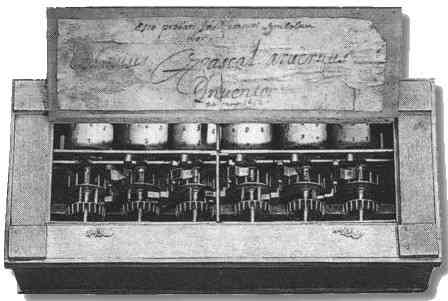
\includegraphics[width=0.4\textwidth]{./EtapaPrimeriza/imagenes/cp.jpg}
  \caption{Calculadora Pascalina (\href{https://www.tispain.com/2014/11/la-pascalina-la-primera-calculadora.html} {Primera Calculadora})}
  \label{cp}
\end{center}
\end{figure}

La máquina estaba compuesta de 8 ruedas dentadas conectadas entre sí con una numeración en ellas de 0 a 9 y una manivela que en función de de la forma de girarla indicaba la operación matemática que se quería realizar. Las 8 ruedas estaban distribuidas de la siguiente manera: dos de ellas se dedicaban a número decimales y las 6 restantes se utilizaban para números enteros. Esto significa que la calculadora te permitía hacer operaciones con número entre 0,01 y 999.999,99 lo que facilitaba un amplio rango de operaciones.\\

Lo curioso recae en el cómo se le ocurrió al joven Pascal inventar la calculadora. Era hijo de un funcionario recaudador de impuesto y en numerosas ocasiones ayudaba a su padre a redactar informes oficiales. Pascal pensó que si conseguía crear una calculadora ahorraría mucho tiempo y al mismo tiempo se aseguraba que los resultados eran correctos. Como resultado de ello apareció la primera calculadora mecánica de la historia dejando atrás instrumentos para contar como puede ser el ábaco.
